% SOURCE: submissions/d2-neurocomputing/zenodo-deposit/results/merging/RG_crossterm_alignment_ALL_REFIX20260801.json :: bundles.*.cells.g2_s{0,1,2}.rho_proj_drop (sign split by regime from submissions/d2-neurocomputing/zenodo-deposit/results/merging/RG_gain_law_MERGED_REFIX20260730.json :: bundles.*.gain_median_absdrop_per_dose vs cut 8)
% !TEX encoding = UTF-8 Unicode
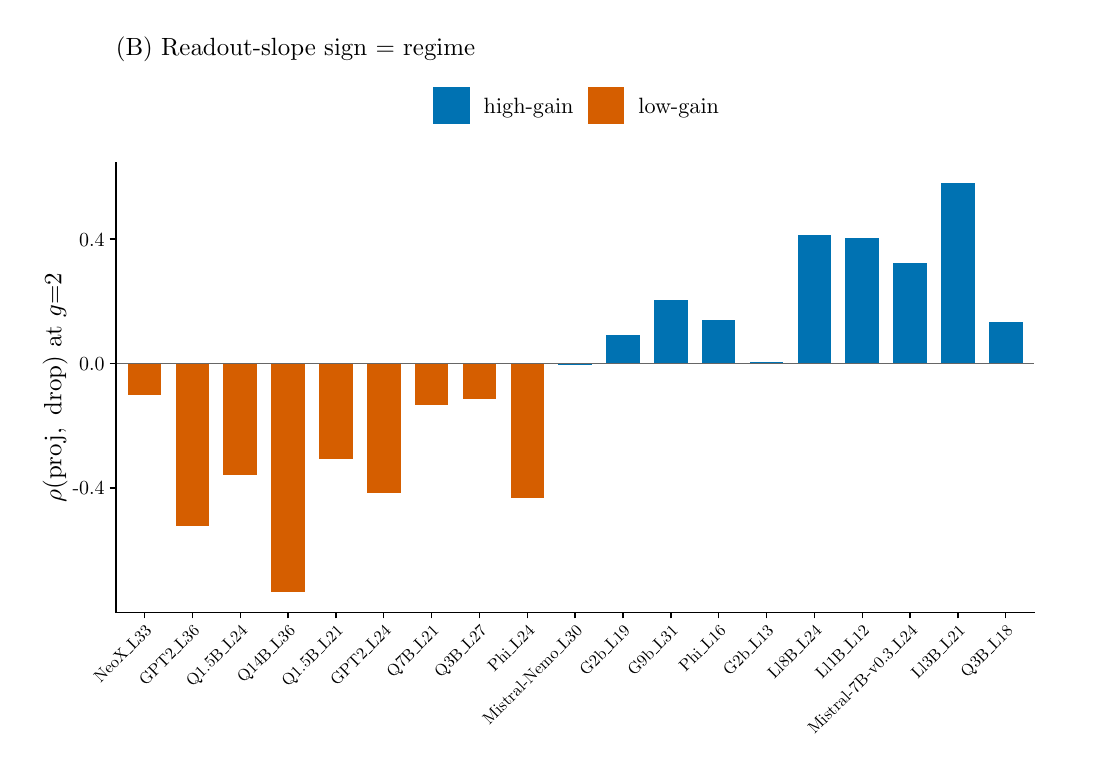
\begin{tikzpicture}[x=1pt,y=1pt]
\definecolor{fillColor}{RGB}{255,255,255}
\path[use as bounding box,fill=fillColor,fill opacity=0.00] (0,0) rectangle (375.80,260.17);
\begin{scope}
\path[clip] (  0.00,  0.00) rectangle (375.80,260.17);
\definecolor{drawColor}{RGB}{255,255,255}
\definecolor{fillColor}{RGB}{255,255,255}

\path[draw=drawColor,line width= 0.5pt,line join=round,line cap=round,fill=fillColor] (  0.00,  0.00) rectangle (375.80,260.17);
\end{scope}
\begin{scope}
\path[clip] ( 31.85, 48.95) rectangle (363.80,211.27);
\definecolor{fillColor}{RGB}{255,255,255}

\path[fill=fillColor] ( 31.85, 48.95) rectangle (363.80,211.27);
\definecolor{fillColor}{RGB}{213,94,0}

\path[fill=fillColor] ( 36.17,127.30) rectangle ( 48.27,138.80);

\path[fill=fillColor] ( 53.46, 80.10) rectangle ( 65.56,138.80);

\path[fill=fillColor] ( 70.75, 98.60) rectangle ( 82.85,138.80);

\path[fill=fillColor] ( 88.04, 56.33) rectangle (100.14,138.80);

\path[fill=fillColor] (105.33,104.38) rectangle (117.43,138.80);

\path[fill=fillColor] (122.62, 92.07) rectangle (134.72,138.80);

\path[fill=fillColor] (139.90,123.79) rectangle (152.01,138.80);

\path[fill=fillColor] (157.19,125.86) rectangle (169.30,138.80);

\path[fill=fillColor] (174.48, 90.11) rectangle (186.59,138.80);
\definecolor{fillColor}{RGB}{0,114,178}

\path[fill=fillColor] (191.77,138.12) rectangle (203.88,138.80);

\path[fill=fillColor] (209.06,138.80) rectangle (221.17,148.95);

\path[fill=fillColor] (226.35,138.80) rectangle (238.45,161.93);

\path[fill=fillColor] (243.64,138.80) rectangle (255.74,154.44);

\path[fill=fillColor] (260.93,138.80) rectangle (273.03,139.45);

\path[fill=fillColor] (278.22,138.80) rectangle (290.32,185.24);

\path[fill=fillColor] (295.51,138.80) rectangle (307.61,184.20);

\path[fill=fillColor] (312.80,138.80) rectangle (324.90,175.09);

\path[fill=fillColor] (330.09,138.80) rectangle (342.19,203.89);

\path[fill=fillColor] (347.38,138.80) rectangle (359.48,153.72);
\definecolor{drawColor}{gray}{0.40}

\path[draw=drawColor,line width= 0.5pt,line join=round] ( 31.85,138.80) -- (363.80,138.80);
\end{scope}
\begin{scope}
\path[clip] (  0.00,  0.00) rectangle (375.80,260.17);
\definecolor{drawColor}{RGB}{0,0,0}

\path[draw=drawColor,line width= 0.5pt,line join=round,line cap=rect] ( 31.85, 48.95) --
	( 31.85,211.27);
\end{scope}
\begin{scope}
\path[clip] (  0.00,  0.00) rectangle (375.80,260.17);
\definecolor{drawColor}{RGB}{0,0,0}

\node[text=drawColor,anchor=base east,inner sep=0pt, outer sep=0pt, scale=  0.72] at ( 27.80, 91.38) {-0.4};

\node[text=drawColor,anchor=base east,inner sep=0pt, outer sep=0pt, scale=  0.72] at ( 27.80,136.32) {0.0};

\node[text=drawColor,anchor=base east,inner sep=0pt, outer sep=0pt, scale=  0.72] at ( 27.80,181.26) {0.4};
\end{scope}
\begin{scope}
\path[clip] (  0.00,  0.00) rectangle (375.80,260.17);
\definecolor{drawColor}{RGB}{0,0,0}

\path[draw=drawColor,line width= 0.5pt,line join=round] ( 29.60, 93.86) --
	( 31.85, 93.86);

\path[draw=drawColor,line width= 0.5pt,line join=round] ( 29.60,138.80) --
	( 31.85,138.80);

\path[draw=drawColor,line width= 0.5pt,line join=round] ( 29.60,183.74) --
	( 31.85,183.74);
\end{scope}
\begin{scope}
\path[clip] (  0.00,  0.00) rectangle (375.80,260.17);
\definecolor{drawColor}{RGB}{0,0,0}

\path[draw=drawColor,line width= 0.5pt,line join=round,line cap=rect] ( 31.85, 48.95) --
	(363.80, 48.95);
\end{scope}
\begin{scope}
\path[clip] (  0.00,  0.00) rectangle (375.80,260.17);
\definecolor{drawColor}{RGB}{0,0,0}

\path[draw=drawColor,line width= 0.5pt,line join=round] ( 42.22, 46.70) --
	( 42.22, 48.95);

\path[draw=drawColor,line width= 0.5pt,line join=round] ( 59.51, 46.70) --
	( 59.51, 48.95);

\path[draw=drawColor,line width= 0.5pt,line join=round] ( 76.80, 46.70) --
	( 76.80, 48.95);

\path[draw=drawColor,line width= 0.5pt,line join=round] ( 94.09, 46.70) --
	( 94.09, 48.95);

\path[draw=drawColor,line width= 0.5pt,line join=round] (111.38, 46.70) --
	(111.38, 48.95);

\path[draw=drawColor,line width= 0.5pt,line join=round] (128.67, 46.70) --
	(128.67, 48.95);

\path[draw=drawColor,line width= 0.5pt,line join=round] (145.96, 46.70) --
	(145.96, 48.95);

\path[draw=drawColor,line width= 0.5pt,line join=round] (163.25, 46.70) --
	(163.25, 48.95);

\path[draw=drawColor,line width= 0.5pt,line join=round] (180.54, 46.70) --
	(180.54, 48.95);

\path[draw=drawColor,line width= 0.5pt,line join=round] (197.82, 46.70) --
	(197.82, 48.95);

\path[draw=drawColor,line width= 0.5pt,line join=round] (215.11, 46.70) --
	(215.11, 48.95);

\path[draw=drawColor,line width= 0.5pt,line join=round] (232.40, 46.70) --
	(232.40, 48.95);

\path[draw=drawColor,line width= 0.5pt,line join=round] (249.69, 46.70) --
	(249.69, 48.95);

\path[draw=drawColor,line width= 0.5pt,line join=round] (266.98, 46.70) --
	(266.98, 48.95);

\path[draw=drawColor,line width= 0.5pt,line join=round] (284.27, 46.70) --
	(284.27, 48.95);

\path[draw=drawColor,line width= 0.5pt,line join=round] (301.56, 46.70) --
	(301.56, 48.95);

\path[draw=drawColor,line width= 0.5pt,line join=round] (318.85, 46.70) --
	(318.85, 48.95);

\path[draw=drawColor,line width= 0.5pt,line join=round] (336.14, 46.70) --
	(336.14, 48.95);

\path[draw=drawColor,line width= 0.5pt,line join=round] (353.43, 46.70) --
	(353.43, 48.95);
\end{scope}
\begin{scope}
\path[clip] (  0.00,  0.00) rectangle (375.80,260.17);
\definecolor{drawColor}{RGB}{0,0,0}

\node[text=drawColor,rotate= 45.00,anchor=base east,inner sep=0pt, outer sep=0pt, scale=  0.60] at ( 45.14, 41.98) {NeoX\_L33};

\node[text=drawColor,rotate= 45.00,anchor=base east,inner sep=0pt, outer sep=0pt, scale=  0.60] at ( 62.43, 41.98) {GPT2\_L36};

\node[text=drawColor,rotate= 45.00,anchor=base east,inner sep=0pt, outer sep=0pt, scale=  0.60] at ( 79.72, 41.98) {Q1.5B\_L24};

\node[text=drawColor,rotate= 45.00,anchor=base east,inner sep=0pt, outer sep=0pt, scale=  0.60] at ( 97.01, 41.98) {Q14B\_L36};

\node[text=drawColor,rotate= 45.00,anchor=base east,inner sep=0pt, outer sep=0pt, scale=  0.60] at (114.30, 41.98) {Q1.5B\_L21};

\node[text=drawColor,rotate= 45.00,anchor=base east,inner sep=0pt, outer sep=0pt, scale=  0.60] at (131.59, 41.98) {GPT2\_L24};

\node[text=drawColor,rotate= 45.00,anchor=base east,inner sep=0pt, outer sep=0pt, scale=  0.60] at (148.88, 41.98) {Q7B\_L21};

\node[text=drawColor,rotate= 45.00,anchor=base east,inner sep=0pt, outer sep=0pt, scale=  0.60] at (166.17, 41.98) {Q3B\_L27};

\node[text=drawColor,rotate= 45.00,anchor=base east,inner sep=0pt, outer sep=0pt, scale=  0.60] at (183.46, 41.98) {Phi\_L24};

\node[text=drawColor,rotate= 45.00,anchor=base east,inner sep=0pt, outer sep=0pt, scale=  0.60] at (200.75, 41.98) {Mistral-Nemo\_L30};

\node[text=drawColor,rotate= 45.00,anchor=base east,inner sep=0pt, outer sep=0pt, scale=  0.60] at (218.04, 41.98) {G2b\_L19};

\node[text=drawColor,rotate= 45.00,anchor=base east,inner sep=0pt, outer sep=0pt, scale=  0.60] at (235.33, 41.98) {G9b\_L31};

\node[text=drawColor,rotate= 45.00,anchor=base east,inner sep=0pt, outer sep=0pt, scale=  0.60] at (252.62, 41.98) {Phi\_L16};

\node[text=drawColor,rotate= 45.00,anchor=base east,inner sep=0pt, outer sep=0pt, scale=  0.60] at (269.90, 41.98) {G2b\_L13};

\node[text=drawColor,rotate= 45.00,anchor=base east,inner sep=0pt, outer sep=0pt, scale=  0.60] at (287.19, 41.98) {Ll8B\_L24};

\node[text=drawColor,rotate= 45.00,anchor=base east,inner sep=0pt, outer sep=0pt, scale=  0.60] at (304.48, 41.98) {Ll1B\_L12};

\node[text=drawColor,rotate= 45.00,anchor=base east,inner sep=0pt, outer sep=0pt, scale=  0.60] at (321.77, 41.98) {Mistral-7B-v0.3\_L24};

\node[text=drawColor,rotate= 45.00,anchor=base east,inner sep=0pt, outer sep=0pt, scale=  0.60] at (339.06, 41.98) {Ll3B\_L21};

\node[text=drawColor,rotate= 45.00,anchor=base east,inner sep=0pt, outer sep=0pt, scale=  0.60] at (356.35, 41.98) {Q3B\_L18};
\end{scope}
\begin{scope}
\path[clip] (  0.00,  0.00) rectangle (375.80,260.17);
\definecolor{drawColor}{RGB}{0,0,0}

\node[text=drawColor,rotate= 90.00,anchor=base,inner sep=0pt, outer sep=0pt, scale=  0.90] at ( 12.20,130.11) {$\rho(\mathrm{proj},\ \mathrm{drop})$ at $g{=}2$};
\end{scope}
\begin{scope}
\path[clip] (  0.00,  0.00) rectangle (375.80,260.17);
\definecolor{fillColor}{RGB}{255,255,255}

\path[fill=fillColor] (141.35,220.27) rectangle (254.30,243.72);
\end{scope}
\begin{scope}
\path[clip] (  0.00,  0.00) rectangle (375.80,260.17);
\definecolor{fillColor}{RGB}{255,255,255}

\path[fill=fillColor] (145.85,224.77) rectangle (160.30,239.22);
\definecolor{fillColor}{RGB}{0,114,178}

\path[fill=fillColor] (146.43,225.35) rectangle (159.72,238.64);
\end{scope}
\begin{scope}
\path[clip] (  0.00,  0.00) rectangle (375.80,260.17);
\definecolor{fillColor}{RGB}{255,255,255}

\path[fill=fillColor] (201.74,224.77) rectangle (216.19,239.22);
\definecolor{fillColor}{RGB}{213,94,0}

\path[fill=fillColor] (202.32,225.35) rectangle (215.61,238.64);
\end{scope}
\begin{scope}
\path[clip] (  0.00,  0.00) rectangle (375.80,260.17);
\definecolor{drawColor}{RGB}{0,0,0}

\node[text=drawColor,anchor=base west,inner sep=0pt, outer sep=0pt, scale=  0.80] at (164.80,229.24) {high-gain};
\end{scope}
\begin{scope}
\path[clip] (  0.00,  0.00) rectangle (375.80,260.17);
\definecolor{drawColor}{RGB}{0,0,0}

\node[text=drawColor,anchor=base west,inner sep=0pt, outer sep=0pt, scale=  0.80] at (220.69,229.24) {low-gain};
\end{scope}
\begin{scope}
\path[clip] (  0.00,  0.00) rectangle (375.80,260.17);
\definecolor{drawColor}{RGB}{0,0,0}

\node[text=drawColor,anchor=base west,inner sep=0pt, outer sep=0pt, scale=  0.90] at ( 31.85,249.97) {(B) Readout-slope sign $=$ regime};
\end{scope}
\end{tikzpicture}
